\documentclass{standalone}
\usepackage{tikz}
\usetikzlibrary{patterns, positioning}
\usepackage[sfdefault]{ClearSans} %% option 'sfdefault' activates Clear Sans as the default text font
\usepackage[T1]{fontenc}

\begin{document}
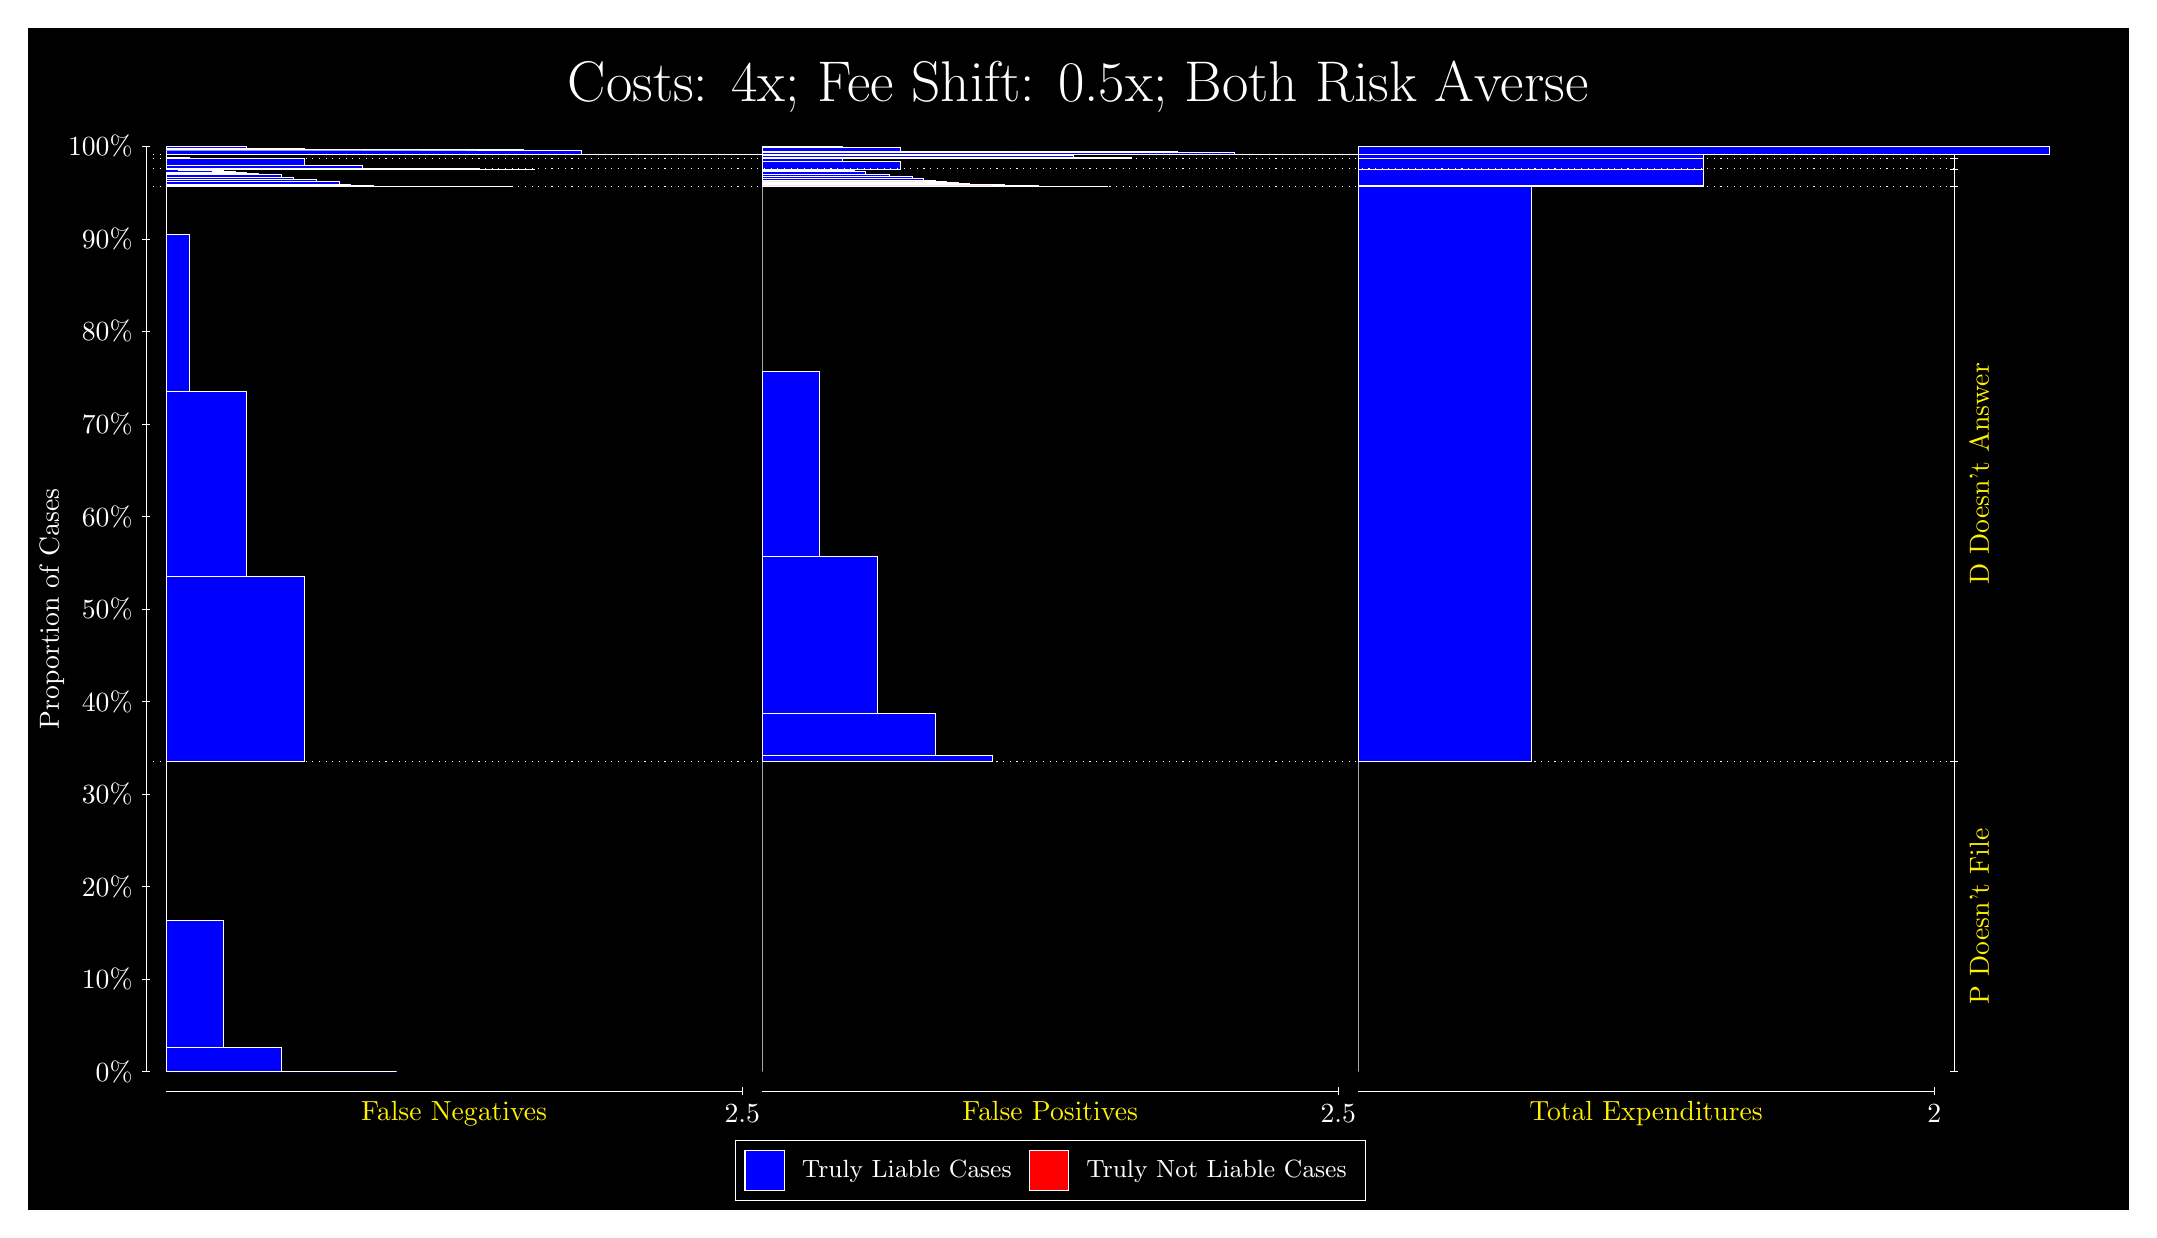
\begin{tikzpicture}
\draw[fill=black] (0,0) rectangle (26.667,15);
\draw[text=white] (0,13.5) rectangle (26.667,15) node[midway] {\huge Costs: 4x; Fee Shift: 0.5x; Both Risk Averse};
\draw[white, very thin] (1.5,1.75) -- (1.5,13.5);
\node[rotate=90, text=white, anchor=center] at (0.3, 7.625) {Proportion of Cases};
\draw[white, very thin] (1.45,1.75) -- (1.55,1.75);
\node[text=white, anchor=east] at (1.45, 1.75) {0\%};
\draw[white, very thin] (1.45,2.925) -- (1.55,2.925);
\node[text=white, anchor=east] at (1.45, 2.925) {10\%};
\draw[white, very thin] (1.45,4.1) -- (1.55,4.1);
\node[text=white, anchor=east] at (1.45, 4.1) {20\%};
\draw[white, very thin] (1.45,5.275) -- (1.55,5.275);
\node[text=white, anchor=east] at (1.45, 5.275) {30\%};
\draw[white, very thin] (1.45,6.45) -- (1.55,6.45);
\node[text=white, anchor=east] at (1.45, 6.45) {40\%};
\draw[white, very thin] (1.45,7.625) -- (1.55,7.625);
\node[text=white, anchor=east] at (1.45, 7.625) {50\%};
\draw[white, very thin] (1.45,8.8) -- (1.55,8.8);
\node[text=white, anchor=east] at (1.45, 8.8) {60\%};
\draw[white, very thin] (1.45,9.975) -- (1.55,9.975);
\node[text=white, anchor=east] at (1.45, 9.975) {70\%};
\draw[white, very thin] (1.45,11.15) -- (1.55,11.15);
\node[text=white, anchor=east] at (1.45, 11.15) {80\%};
\draw[white, very thin] (1.45,12.325) -- (1.55,12.325);
\node[text=white, anchor=east] at (1.45, 12.325) {90\%};
\draw[white, very thin] (1.45,13.5) -- (1.55,13.5);
\node[text=white, anchor=east] at (1.45, 13.5) {100\%};

\draw[white, very thin] (24.457,1.75) -- (24.457,13.5);
\draw[white, very thin] (24.407,1.75) -- (24.507,1.75);
\node[anchor=west] at (24.407, 1.75) {};
\draw[white, very thin] (24.407,5.6883) -- (24.507,5.6883);
\node[anchor=west] at (24.407, 5.6883) {};
\draw[white, very thin] (24.407,12.991) -- (24.507,12.991);
\node[anchor=west] at (24.407, 12.991) {};
\draw[white, very thin] (24.407,13.214) -- (24.507,13.214);
\node[anchor=west] at (24.407, 13.214) {};
\draw[white, very thin] (24.407,13.35) -- (24.507,13.35);
\node[anchor=west] at (24.407, 13.35) {};
\draw[white, very thin] (24.407,13.397) -- (24.507,13.397);
\node[anchor=west] at (24.407, 13.397) {};
\draw[white, very thin] (24.407,13.5) -- (24.507,13.5);
\node[anchor=west] at (24.407, 13.5) {};

\draw[white, very thin, fill=blue] (1.75,1.75) rectangle (4.6775,1.75);
\draw[white, very thin, fill=blue] (1.75,1.75) rectangle (3.9457,1.7526);
\draw[white, very thin, fill=blue] (1.75,1.7526) rectangle (3.2138,2.0544);
\draw[white, very thin, fill=blue] (1.75,2.0544) rectangle (2.4819,3.6756);
\draw[white, very thin, fill=red] (1.75,3.6756) rectangle (1.75,3.6756);
\draw[white, very thin, fill=blue] (1.75,3.6756) rectangle (1.75,5.6883);
\draw[white, very thin, fill=blue] (1.75,5.6883) rectangle (3.5065,8.0382);
\draw[white, very thin, fill=blue] (1.75,8.0382) rectangle (2.7746,10.385);
\draw[white, very thin, fill=blue] (1.75,10.385) rectangle (2.0428,12.378);
\draw[white, very thin, fill=red] (1.75,12.378) rectangle (1.75,12.378);
\draw[white, very thin, fill=blue] (1.75,12.378) rectangle (1.75,12.991);
\draw[white, very thin, fill=blue] (1.75,12.991) rectangle (6.1413,12.991);
\draw[white, very thin, fill=blue] (1.75,12.991) rectangle (5.8486,12.991);
\draw[white, very thin, fill=blue] (1.75,12.991) rectangle (5.5558,12.991);
\draw[white, very thin, fill=blue] (1.75,12.991) rectangle (5.4094,12.992);
\draw[white, very thin, fill=blue] (1.75,12.992) rectangle (5.2631,12.992);
\draw[white, very thin, fill=blue] (1.75,12.992) rectangle (5.1167,12.992);
\draw[white, very thin, fill=blue] (1.75,12.992) rectangle (4.9703,12.992);
\draw[white, very thin, fill=blue] (1.75,12.992) rectangle (4.8239,12.992);
\draw[white, very thin, fill=blue] (1.75,12.992) rectangle (4.6775,12.998);
\draw[white, very thin, fill=blue] (1.75,12.998) rectangle (4.5312,12.998);
\draw[white, very thin, fill=blue] (1.75,12.998) rectangle (4.3848,12.998);
\draw[white, very thin, fill=blue] (1.75,12.998) rectangle (4.3848,13.01);
\draw[white, very thin, fill=blue] (1.75,13.01) rectangle (4.2384,13.01);
\draw[white, very thin, fill=blue] (1.75,13.01) rectangle (4.092,13.018);
\draw[white, very thin, fill=blue] (1.75,13.018) rectangle (4.092,13.018);
\draw[white, very thin, fill=blue] (1.75,13.018) rectangle (3.9457,13.055);
\draw[white, very thin, fill=blue] (1.75,13.055) rectangle (3.7993,13.059);
\draw[white, very thin, fill=blue] (1.75,13.059) rectangle (3.6529,13.059);
\draw[white, very thin, fill=blue] (1.75,13.059) rectangle (3.6529,13.082);
\draw[white, very thin, fill=blue] (1.75,13.082) rectangle (3.5065,13.087);
\draw[white, very thin, fill=blue] (1.75,13.087) rectangle (3.3602,13.106);
\draw[white, very thin, fill=blue] (1.75,13.106) rectangle (3.3602,13.106);
\draw[white, very thin, fill=blue] (1.75,13.106) rectangle (3.2138,13.141);
\draw[white, very thin, fill=blue] (1.75,13.141) rectangle (3.0674,13.145);
\draw[white, very thin, fill=blue] (1.75,13.145) rectangle (3.0674,13.148);
\draw[white, very thin, fill=blue] (1.75,13.148) rectangle (2.921,13.15);
\draw[white, very thin, fill=blue] (1.75,13.15) rectangle (2.921,13.16);
\draw[white, very thin, fill=blue] (1.75,13.16) rectangle (2.7746,13.169);
\draw[white, very thin, fill=blue] (1.75,13.169) rectangle (2.6283,13.186);
\draw[white, very thin, fill=blue] (1.75,13.186) rectangle (2.6283,13.186);
\draw[white, very thin, fill=blue] (1.75,13.186) rectangle (2.4819,13.19);
\draw[white, very thin, fill=blue] (1.75,13.19) rectangle (2.3355,13.192);
\draw[white, very thin, fill=blue] (1.75,13.192) rectangle (2.3355,13.194);
\draw[white, very thin, fill=blue] (1.75,13.194) rectangle (2.1891,13.197);
\draw[white, very thin, fill=blue] (1.75,13.197) rectangle (2.0428,13.203);
\draw[white, very thin, fill=blue] (1.75,13.203) rectangle (1.8964,13.204);
\draw[white, very thin, fill=red] (1.75,13.204) rectangle (1.75,13.204);
\draw[white, very thin, fill=blue] (1.75,13.204) rectangle (1.75,13.214);
\draw[white, very thin, fill=blue] (1.75,13.214) rectangle (6.4341,13.214);
\draw[white, very thin, fill=blue] (1.75,13.214) rectangle (5.7022,13.215);
\draw[white, very thin, fill=blue] (1.75,13.215) rectangle (4.9703,13.219);
\draw[white, very thin, fill=blue] (1.75,13.219) rectangle (4.2384,13.255);
\draw[white, very thin, fill=blue] (1.75,13.255) rectangle (3.5065,13.35);
\draw[white, very thin, fill=red] (1.75,13.35) rectangle (1.75,13.35);
\draw[white, very thin, fill=blue] (1.75,13.35) rectangle (3.5065,13.35);
\draw[white, very thin, fill=blue] (1.75,13.35) rectangle (2.7746,13.351);
\draw[white, very thin, fill=blue] (1.75,13.351) rectangle (2.0428,13.36);
\draw[white, very thin, fill=red] (1.75,13.36) rectangle (1.75,13.36);
\draw[white, very thin, fill=blue] (1.75,13.36) rectangle (1.75,13.397);
\draw[white, very thin, fill=blue] (1.75,13.397) rectangle (9.9471,13.397);
\draw[white, very thin, fill=blue] (1.75,13.397) rectangle (9.2152,13.397);
\draw[white, very thin, fill=blue] (1.75,13.397) rectangle (8.4834,13.397);
\draw[white, very thin, fill=blue] (1.75,13.397) rectangle (7.7515,13.404);
\draw[white, very thin, fill=blue] (1.75,13.404) rectangle (7.0196,13.455);
\draw[white, very thin, fill=blue] (1.75,13.455) rectangle (6.2877,13.458);
\draw[white, very thin, fill=blue] (1.75,13.458) rectangle (5.7022,13.458);
\draw[white, very thin, fill=blue] (1.75,13.458) rectangle (5.5558,13.458);
\draw[white, very thin, fill=blue] (1.75,13.458) rectangle (4.9703,13.458);
\draw[white, very thin, fill=blue] (1.75,13.458) rectangle (4.2384,13.458);
\draw[white, very thin, fill=blue] (1.75,13.458) rectangle (3.5065,13.471);
\draw[white, very thin, fill=blue] (1.75,13.471) rectangle (2.7746,13.497);
\draw[white, very thin, fill=blue] (1.75,13.497) rectangle (2.0428,13.5);
\draw[white, very thin, fill=red] (1.75,13.5) rectangle (1.75,13.5);
\draw[white, very thin, fill=blue] (1.75,13.5) rectangle (1.75,13.5);
\draw[white, very thin, fill=red] (9.3189,1.75) rectangle (9.3189,1.75);
\draw[white, very thin, fill=blue] (9.3189,1.75) rectangle (9.3189,5.6883);
\draw[white, very thin, fill=red] (9.3189,5.6883) rectangle (12.246,5.6883);
\draw[white, very thin, fill=blue] (9.3189,5.6883) rectangle (12.246,5.7616);
\draw[white, very thin, fill=blue] (9.3189,5.7616) rectangle (11.515,6.302);
\draw[white, very thin, fill=blue] (9.3189,6.302) rectangle (10.783,8.2946);
\draw[white, very thin, fill=blue] (9.3189,8.2946) rectangle (10.051,10.642);
\draw[white, very thin, fill=blue] (9.3189,10.642) rectangle (9.3189,12.991);
\draw[white, very thin, fill=red] (9.3189,12.991) rectangle (13.71,12.991);
\draw[white, very thin, fill=blue] (9.3189,12.991) rectangle (13.71,12.993);
\draw[white, very thin, fill=red] (9.3189,12.993) rectangle (13.417,12.993);
\draw[white, very thin, fill=blue] (9.3189,12.993) rectangle (13.417,12.994);
\draw[white, very thin, fill=red] (9.3189,12.994) rectangle (13.125,12.994);
\draw[white, very thin, fill=blue] (9.3189,12.994) rectangle (13.125,12.997);
\draw[white, very thin, fill=blue] (9.3189,12.997) rectangle (12.978,12.998);
\draw[white, very thin, fill=red] (9.3189,12.998) rectangle (12.832,12.998);
\draw[white, very thin, fill=blue] (9.3189,12.998) rectangle (12.832,13.002);
\draw[white, very thin, fill=blue] (9.3189,13.002) rectangle (12.686,13.003);
\draw[white, very thin, fill=red] (9.3189,13.003) rectangle (12.539,13.003);
\draw[white, very thin, fill=blue] (9.3189,13.003) rectangle (12.539,13.009);
\draw[white, very thin, fill=blue] (9.3189,13.009) rectangle (12.393,13.012);
\draw[white, very thin, fill=red] (9.3189,13.012) rectangle (12.246,13.012);
\draw[white, very thin, fill=blue] (9.3189,13.012) rectangle (12.246,13.016);
\draw[white, very thin, fill=blue] (9.3189,13.016) rectangle (12.1,13.02);
\draw[white, very thin, fill=red] (9.3189,13.02) rectangle (11.954,13.02);
\draw[white, very thin, fill=blue] (9.3189,13.02) rectangle (11.954,13.037);
\draw[white, very thin, fill=blue] (9.3189,13.037) rectangle (11.807,13.046);
\draw[white, very thin, fill=red] (9.3189,13.046) rectangle (11.661,13.046);
\draw[white, very thin, fill=blue] (9.3189,13.046) rectangle (11.661,13.056);
\draw[white, very thin, fill=blue] (9.3189,13.056) rectangle (11.661,13.058);
\draw[white, very thin, fill=blue] (9.3189,13.058) rectangle (11.515,13.065);
\draw[white, very thin, fill=red] (9.3189,13.065) rectangle (11.368,13.065);
\draw[white, very thin, fill=blue] (9.3189,13.065) rectangle (11.368,13.1);
\draw[white, very thin, fill=blue] (9.3189,13.1) rectangle (11.222,13.119);
\draw[white, very thin, fill=blue] (9.3189,13.119) rectangle (11.075,13.124);
\draw[white, very thin, fill=blue] (9.3189,13.124) rectangle (10.929,13.147);
\draw[white, very thin, fill=blue] (9.3189,13.147) rectangle (10.929,13.147);
\draw[white, very thin, fill=blue] (9.3189,13.147) rectangle (10.783,13.151);
\draw[white, very thin, fill=blue] (9.3189,13.151) rectangle (10.636,13.188);
\draw[white, very thin, fill=blue] (9.3189,13.188) rectangle (10.49,13.196);
\draw[white, very thin, fill=blue] (9.3189,13.196) rectangle (10.344,13.196);
\draw[white, very thin, fill=blue] (9.3189,13.196) rectangle (10.197,13.208);
\draw[white, very thin, fill=blue] (9.3189,13.208) rectangle (10.197,13.208);
\draw[white, very thin, fill=blue] (9.3189,13.208) rectangle (10.051,13.208);
\draw[white, very thin, fill=blue] (9.3189,13.208) rectangle (9.9044,13.214);
\draw[white, very thin, fill=blue] (9.3189,13.214) rectangle (9.758,13.214);
\draw[white, very thin, fill=blue] (9.3189,13.214) rectangle (9.6116,13.214);
\draw[white, very thin, fill=blue] (9.3189,13.214) rectangle (9.4652,13.214);
\draw[white, very thin, fill=blue] (9.3189,13.214) rectangle (9.3189,13.214);
\draw[white, very thin, fill=red] (9.3189,13.214) rectangle (11.075,13.214);
\draw[white, very thin, fill=blue] (9.3189,13.214) rectangle (11.075,13.309);
\draw[white, very thin, fill=blue] (9.3189,13.309) rectangle (10.344,13.346);
\draw[white, very thin, fill=blue] (9.3189,13.346) rectangle (9.6116,13.35);
\draw[white, very thin, fill=blue] (9.3189,13.35) rectangle (9.3189,13.35);
\draw[white, very thin, fill=red] (9.3189,13.35) rectangle (14.003,13.35);
\draw[white, very thin, fill=blue] (9.3189,13.35) rectangle (14.003,13.367);
\draw[white, very thin, fill=blue] (9.3189,13.367) rectangle (13.271,13.387);
\draw[white, very thin, fill=blue] (9.3189,13.387) rectangle (12.539,13.397);
\draw[white, very thin, fill=blue] (9.3189,13.397) rectangle (11.807,13.397);
\draw[white, very thin, fill=blue] (9.3189,13.397) rectangle (11.075,13.397);
\draw[white, very thin, fill=red] (9.3189,13.397) rectangle (17.516,13.397);
\draw[white, very thin, fill=blue] (9.3189,13.397) rectangle (17.516,13.397);
\draw[white, very thin, fill=red] (9.3189,13.397) rectangle (16.784,13.397);
\draw[white, very thin, fill=blue] (9.3189,13.397) rectangle (16.784,13.397);
\draw[white, very thin, fill=red] (9.3189,13.397) rectangle (16.052,13.397);
\draw[white, very thin, fill=blue] (9.3189,13.397) rectangle (16.052,13.4);
\draw[white, very thin, fill=red] (9.3189,13.4) rectangle (15.32,13.4);
\draw[white, very thin, fill=blue] (9.3189,13.4) rectangle (15.32,13.427);
\draw[white, very thin, fill=blue] (9.3189,13.427) rectangle (14.588,13.439);
\draw[white, very thin, fill=blue] (9.3189,13.439) rectangle (13.857,13.439);
\draw[white, very thin, fill=blue] (9.3189,13.439) rectangle (13.125,13.439);
\draw[white, very thin, fill=red] (9.3189,13.439) rectangle (12.539,13.439);
\draw[white, very thin, fill=blue] (9.3189,13.439) rectangle (12.539,13.439);
\draw[white, very thin, fill=blue] (9.3189,13.439) rectangle (12.393,13.439);
\draw[white, very thin, fill=blue] (9.3189,13.439) rectangle (11.807,13.44);
\draw[white, very thin, fill=red] (9.3189,13.44) rectangle (11.807,13.44);
\draw[white, very thin, fill=blue] (9.3189,13.44) rectangle (11.807,13.442);
\draw[white, very thin, fill=blue] (9.3189,13.442) rectangle (11.075,13.443);
\draw[white, very thin, fill=red] (9.3189,13.443) rectangle (11.075,13.443);
\draw[white, very thin, fill=blue] (9.3189,13.443) rectangle (11.075,13.493);
\draw[white, very thin, fill=blue] (9.3189,13.493) rectangle (10.344,13.493);
\draw[white, very thin, fill=blue] (9.3189,13.493) rectangle (10.344,13.5);
\draw[white, very thin, fill=blue] (9.3189,13.5) rectangle (9.6116,13.5);
\draw[white, very thin, fill=blue] (9.3189,13.5) rectangle (9.6116,13.5);
\draw[white, very thin, fill=blue] (9.3189,13.5) rectangle (9.3189,13.5);
\draw[white, very thin, fill=red] (16.888,1.75) rectangle (16.888,1.75);
\draw[white, very thin, fill=blue] (16.888,1.75) rectangle (16.888,5.6883);
\draw[white, very thin, fill=red] (16.888,5.6883) rectangle (19.083,5.6883);
\draw[white, very thin, fill=blue] (16.888,5.6883) rectangle (19.083,12.991);
\draw[white, very thin, fill=red] (16.888,12.991) rectangle (21.279,12.991);
\draw[white, very thin, fill=blue] (16.888,12.991) rectangle (21.279,13.011);
\draw[white, very thin, fill=red] (16.888,13.011) rectangle (21.279,13.011);
\draw[white, very thin, fill=blue] (16.888,13.011) rectangle (21.279,13.204);
\draw[white, very thin, fill=red] (16.888,13.204) rectangle (21.279,13.204);
\draw[white, very thin, fill=blue] (16.888,13.204) rectangle (21.279,13.214);
\draw[white, very thin, fill=red] (16.888,13.214) rectangle (21.279,13.214);
\draw[white, very thin, fill=blue] (16.888,13.214) rectangle (21.279,13.35);
\draw[white, very thin, fill=red] (16.888,13.35) rectangle (21.279,13.35);
\draw[white, very thin, fill=blue] (16.888,13.35) rectangle (21.279,13.397);
\draw[white, very thin, fill=red] (16.888,13.397) rectangle (25.67,13.397);
\draw[white, very thin, fill=blue] (16.888,13.397) rectangle (25.67,13.5);
\draw[white, dotted] (1.5,5.6883) -- (24.457,5.6883);
\draw[white, dotted] (1.5,12.991) -- (24.457,12.991);
\draw[white, dotted] (1.5,13.214) -- (24.457,13.214);
\draw[white, dotted] (1.5,13.35) -- (24.457,13.35);
\draw[white, dotted] (1.5,13.397) -- (24.457,13.397);
\draw[white, very thin] (1.75,1.5) -- (9.0689,1.5);
\node[text=yellow, anchor=north] at (5.4094, 1.5) {False Negatives};
\draw[white, very thin] (9.0689,1.45) -- (9.0689,1.55);
\node[text=white, anchor=north] at (9.0689, 1.45) {2.5};

\draw[white, very thin] (9.3189,1.5) -- (16.638,1.5);
\node[text=yellow, anchor=north] at (12.978, 1.5) {False Positives};
\draw[white, very thin] (16.638,1.45) -- (16.638,1.55);
\node[text=white, anchor=north] at (16.638, 1.45) {2.5};

\draw[white, very thin] (16.888,1.5) -- (24.207,1.5);
\node[text=yellow, anchor=north] at (20.547, 1.5) {Total Expenditures};
\draw[white, very thin] (24.207,1.45) -- (24.207,1.55);
\node[text=white, anchor=north] at (24.207, 1.45) {2};

\node[text=yellow, centered, rotate=90] at (24.777, 3.7191) {P Doesn't File};
\node[text=yellow, centered, rotate=90] at (24.777, 9.3399) {D Doesn't Answer};





\draw (12.978300999999998,1.5) node[draw=none] (baseCoordinate) {};
\begin{scope}[align=center]
        \matrix[scale=0.5, draw=white, below=0.5cm of baseCoordinate, nodes={draw}, column sep=0.1cm]{
            \node[rectangle, draw, minimum width=0.5cm, minimum height=0.5cm, fill=blue] {}; &
            \node[draw=none, font=\small, text=white] (B) {Truly Liable Cases}; &
            \node[rectangle, draw, minimum width=0.5cm, minimum height=0.5cm, fill=red] {}; &
            \node[draw=none, font=\small, text=white] (B) {Truly Not Liable Cases}; \\
            };
\end{scope}

\end{tikzpicture}
\end{document}